\documentclass[a4paper,10pt]{article}
\pagestyle{headings}
\usepackage[T1]{fontenc}
\usepackage[utf8]{inputenc}
\usepackage[francais]{babel}
\usepackage{fullpage}
\usepackage{amsmath}
\usepackage{amssymb}
\usepackage{titling}
\usepackage{graphicx}
\usepackage{titlesec}
%\usepackage[Sonny]{fncychap}
\usepackage[squaren, Gray, cdot]{SIunits}
\usepackage{color}
\usepackage{fancyhdr}
\usepackage{float}
\usepackage{chngpage}
\usepackage[colorlinks=true]{hyperref}

\titleformat*{\section}{\normalfont\bfseries\Large\sf}
\titleformat*{\subsection}{\normalfont\bfseries\large\sf}
\titleformat*{\subsubsection}{\normalfont\bfseries\normalsize\sf}

\newcommand{\HRule}{\rule{\linewidth}{0.3mm}}


\begin{document}
\sffamily
    \begin{titlepage}
        \begin{sffamily}
        \begin{center}
    
        \textsc{\Large Institut National des Sciences Appliquées de Toulouse}\\[5.5cm]
    
        \LARGE Robotique de Service\\[1.5cm]
    
        % Title
        \HRule \\[0.5cm]
        { \huge La robotique de service en général : origines, techniques et avenir\\[0.4cm] }
    
        \HRule \\[4cm]
        \vfill
    
       \begin{minipage}{0.4\textwidth}
          \begin{flushleft} \large
            Johan Medrano\\
            5SIEC
          \end{flushleft}
       \end{minipage}
       \begin{minipage}{0.4\textwidth}
          \begin{flushright} \large
            Pierre Dauchez\\
            \today
          \end{flushright}
       \end{minipage}
    
        \end{center}
        \end{sffamily}
    \end{titlepage}
    
    \tableofcontents
    \newpage
    
    \section*{Introduction}
    
        \paragraph{}
            La robotique constitue un domaine vaste, initialement tiré d'affabulations 
            humaines pour lesquelles l'industrie et la société a pu trouver de l'intérêt. 
            
        \paragraph{}
            Le CNRTL (\textit{Centre National de Ressources Textuelles et Lexicales}) donne la définition 
            suivante du terme \textit{robot} : 
            
        \begin{quote}
            "Appareil effectuant, grâce à un système de commande automatique à base de micro-processeur,
            une tâche précise pour laquelle il a été conçu dans le domaine industriel, scientifique ou domestique."
        \end{quote}
        
        \paragraph{}
            On trouve dans cette définition une notion d'interaction avec l'environnement : le 
            robot est un système complexe et interdisciplinaire, un acteur qui perçoit des informations 
            de son environnement, et les traite de manière à réagir avec une action cohérente. 
            
        \paragraph{}
            Si cette réaction peut être perçue comme une forme d'intelligence, ce n'est pas initialement 
            le but du robot. Originellement dénommé par le mot tchèque "robota", signifiant une "corvée", 
            le robot est censé rester un être servile, alter-ego de l'Homme que ce dernier utilise pour 
            effectuer des tâches qu'il ne souhaite pas ou n'est pas en mesure d'effectuer. 
            
        \paragraph{}
            Ainsi, le robot conquiert son environnement : à la fois sur terre, en mer ou dans les airs, 
            il peut être doté de la capacité de se déplacer. 
            Certains sont également capable de manipuler des objets, et ce avec une précision ou une force
            surhumaine. 
            
        \paragraph{}
            Ces capacités surhumaines ont, depuis le début de l'ère informatique, succité l'engouement 
            des communautés scientifique et industrielle, cette dernière réalisant fréquemment des investissements 
            considérables pour accélérer les progrès du domaine. 
            
        \paragraph{}
            De nos jours, les prémices de l'ère de l'intelligence artificielle annoncent à la fois
            un avenir radieux pour la robotique, mais également de forts problèmes éthique à résoudre. 
            
        \paragraph{}
            Le plan de ce document est à la fois thématique et chronologique : 
                \begin{itemize}
                    \item dans une première partie, il sera question des origines de la robotique et
                    de ses racines ancrées dans la science-fiction, 
                    \item les parties 2 et 3 traiteront de parties plus techniques de la robotique
                    mobile et des manipulateurs
                    \item dans la dernière partie, nous aborderons l'intelligence artificielle 
                    et ce qu'elle peut apporter (et apporte déjà) à la robotique. 
                \end{itemize}
                
    \newpage
    
    \begin{figure}
                
        \centering
        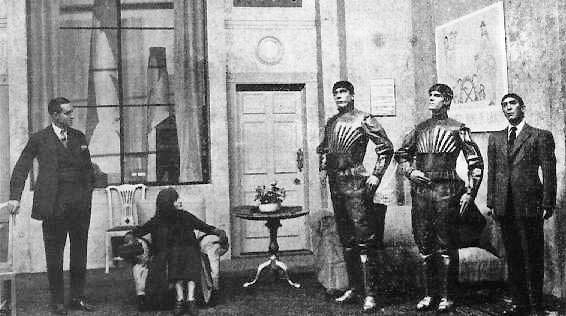
\includegraphics[width=\textwidth]{Capek_play.jpg}
        \caption{La pièce de Capek mise en scène.}
        \label{fig:capekplay}
    \end{figure}
            

    \section{La robotique, une affaire de science fiction : mythe de Frankenstein, Prométhée et Golem} 
        \subsection{\textit{Rossumovi univerzální roboti} (Rossum's Universal Robots, 1920)}
            
            \paragraph{}
                Le terme "robot" apparaît après 1920, suite à la pièce de théâtre 
                de l'auteur tchécoslovaque Carel Čapek. Dans sa pièce \textit{Rossumovi univerzální roboti}
                (Rossum's Universal Robots en anglais), il met en scène des créatures artificielles
                similaires à l'être humain, fabriquées par ce dernier pour réaliser des tâches 
                de production et d'exploitation. Celles-ci sont dénommées par le mot tchèque "\textit{robota}", 
                qui peut être traduit comme "\textit{corvée}" ("\textit{rob}" signifiant \textit{esclave}). 
                
            
            
            \paragraph{}
                Dans le déroulement de la pièce, les robots originellement insensibles et limités se voient 
                dotés par un ingénieur de sentiments simples et d'une intelligence développée. 
                Ils se retournent alors contre la main d'un homme devenu inactif et impuissant, et 
                deviennent maîtres de l'humanité. 
                
            \paragraph{}
                Cette pièce, apparue aux prémices de la robotique, en dresse d'ores et déjà les potentielles 
                conséquences négatives pour l'humain. 
                
        \subsection{L'homme et son \textit{alter ego} dans la fiction} 
            \paragraph{}
                Si Carel Čapek est le premier à introduire le terme "robot", il n'est néanmoins pas le 
                premier à aborder le thème de la vie artificiellement créée des mains de l'Homme.  
                
            \paragraph{} 
                Dans la mythologie grecque, il est possible trouver ce thème dans le 
                mythe de Prométhée. Titan créé par l'Homme, il apporte à ce dernier la 
                technique. Et que dire de Pygmalion, la sculture qui prend vie lorsque 
                son créateur Galatée en tombe amoureux ? 
                
            \paragraph{}
                Plus tard dans l'Histoire, l'humain conçoit des automates et 
                marionnettes qu'il actionne pour insuffler un semblant de vie
                artificielle. 
            
            \paragraph{}
                Les exemples précédents nous montrent qu'il a toujours été 
                dans l'idée de l'Homme de créer des êtres dotés de vie artificielle. 
                L romans \textit{Frankenstein} (1818) et \textit{Le prométhée moderne} (1831)
                de l'écrivaine anglaise Mary Shelley  reprennent également 
                ce thème. 
            
                
            
    \section{Le robotique en général et ses applications}
        \subsection{Robotique manufacturière et robotique de service}
            \paragraph{}
                Lorsque l'on analyse les besoins humains qui nous amènent à 
                construire des robots, on se rend compte que l'on peut les 
                diviser en deux sections : ce qui est de la robotique manufacturière, 
                et vise à utiliser des automates pour de la production, et ce qui ne 
                l'est pas, et qui est généralement regroupé sous la notion commune de 
                robotique de service. 
                
            \paragraph{}
                La robotique manufacturière regroupe une grande partie des 
                robots qui ont été créés pour les besoins de l'industrie et de 
                la production de masse. Ce sont des machines qui effectuent 
                généralement une tâche répétitive, dont l'exercice par l'humain 
                ne présente pas d'intérêt en terme de coût, de vitesse d'exécution, 
                ni même d'intérêt "intellectuel". 
                
            \paragraph{}
                Après la seconde guerre mondiale, pendant la période des 
                Trente Glorieuses, l'opulence des états (et entreprises) victorieux
                permet de forts investissements dans le domaine de la robotique. 
                Avec l'augmentation du pouvoir d'achat des ménages et une augmentation
                massive de la consommation, on a besoin de produire plus, plus vite et 
                à moindre coût : ceci engrange l'aire de l'automatisation. 
                
            \paragraph{}
                L'ouvrier est alors remplacé par des machines, moins chères et plus efficaces.
                Ceci commence en 1961, lorsque le géant de l'automobile General Motors 
                utilise pour la première fois un robot dans ses chaînes d'assemblage.
                Depuis, le nombre de robots industriels en circulation ne cesse
                d'augmenter. 
                
            \paragraph{}
                D'un autre côté, le domaine de la robotique de service regroupe
                tout ce qui n'est pas de la robotique manufacturière. C'est donc 
                le cas des applications utilisant la robotique pour répondre à des 
                besoins humains, comme la robotique médicale, les exosquelettes, 
                l'accueil de personnes dans des lieux particuliers, ... 
                
                    
        \subsection{Une notion commune : les degrés de liberté}
            \paragraph{}
                Nous allons maintenant aborder une notion qui se partage 
                entre tous les domaines de la robotique, à savoir les degrés 
                de liberté. 
        
            \paragraph{}
                En mécanique, un corps peut subir six transformations 
                dans l'espace : trois translations et trois rotations
                selon des axes fixes (ces axes doivent nécessairement former 
                une base de notre espace en 3 dimensions).
                
            \paragraph{}
                Pour un corps indépendant dans l'espace, ces translations 
                et rotations sont quantitativement libres : ce corps a donc 
                6 degrés de liberté. 
        
            \paragraph{}
                De tels corps peuvent être reliés au sein d'une chaîne cinématique 
                grâce à des liaisons mécaniques. Celles-ci imposent des contraintes 
                de translation ou de rotation relatives au reste de la chaîne. Les 
                degrés de liberté d'un corps par rapport à un autre sont alors 
                les mouvements non contraints par la liaison mécanique. 
                
            \paragraph{}
                Prenons l'exemple d'un ustensile commun : le casse-noix. Celui-ci est composé de 
                deux pièces de métal reliées par une liaison pivot. Ces deux pièces de métal, 
                considérées sans la liaison mécanique, sont des solides dans l'espace, et 
                possèdent donc 6 degrés de liberté. 
            
            \paragraph{}
                Cependant, la liaison pivot contraint le mouvement
                des pièces relativement l'une à l'autre : seule la rotation d'une pièce selon
                l'axe de la liaison pivot reste possible. Le nombre de degré de liberté 
                est le nombre de mouvements possibles d'une pièce indépendamment de l'autre, 
                soit un seul pour le casse-noix.
                
            \paragraph{}
                Le nombre de degrés de liberté que possède un robot influe sur sa capacité à 
                interagir avec l'environnement. 
                
            \paragraph{}
                Pour un robot manipulateur possédant un organe terminal, le nombre de 
                degrés de liberté de cet organe sera inférieur ou égal au nombre de degrés de liberté 
                des chaînes cinématiques reliant l'organe à la base. 
                
            \paragraph{}
                Le nombre de degrés de liberté d'un robot mobile influera sur sa 
                capacité à se mouvoir d'une position à une autre sans manoeuvre. 
                Par exemple, un robot mobile terrestre possédant 3 degrés de liberté 
                pourra se déplacer librement sur ses axes transversal et longitudinal 
                et tourner selon son axe vertical. Pour une évolution sur un plan comme
                le sol, le robot pourra atteindre n'importe quelle position, et ce sans manoeuvrer.  
                
        
        

        \subsection{Des applications directes de la robotique de service dans le domaine médical} 
            \subsubsection{Da Vinci}
                \paragraph{}
                    Dans le domaine médical, en perpétuelle évolution, la robotique a pu trouver 
                    une place. En effet, la technologie s'améliore mais les médecins ont toujours 
                    besoin d'instruments plus petits, plus précis et plus fiables pour assurer 
                    leurs opérations. 
                    
                \paragraph{}
                    À cet effet, le robot Da Vinci a été construit par la société américaine
                    \textit{Intuitive Surgical}. Ce robot est téléopéré par un chirurgien, 
                    et permet de réaliser des opérations lourdes avec des outils miniaturisés, 
                    dont il contrôle totallement la chaîne l'actionnement. 
                
                \paragraph{}
                    Des caméras lui permettent de s'immerger totalement dans le corps du 
                    patient, et des interfaces de manipulation lui permettent d'actionner 
                    très précisément les organes terminaux du robot. 
                    
                \paragraph{}
                    Grâce à cela, Da Vinci peut réaliser des opérations risquées, dont 
                    l'empreinte extérieure sur le corps du patient sera réduite par 
                    rapport à celle laissée par une opération chirurgicale classique. 
                    
                \paragraph{}
                    Ce robot peut également être téléopéré à distance. Dans des domaines 
                    très spécifiques de la médecine, seuls un faible nombre de chirurgiens 
                    sont capable de réaliser certaines opérations. Cette téléopération
                    à distance du robot Da Vinci permet à des chirurgiens de réaliser les
                    opérations pour lesquels ils sont spécialistes et ce, quelque soit la position
                    géographique du patient.

                
                
                 \begin{figure}[h!]
                     \centering
                     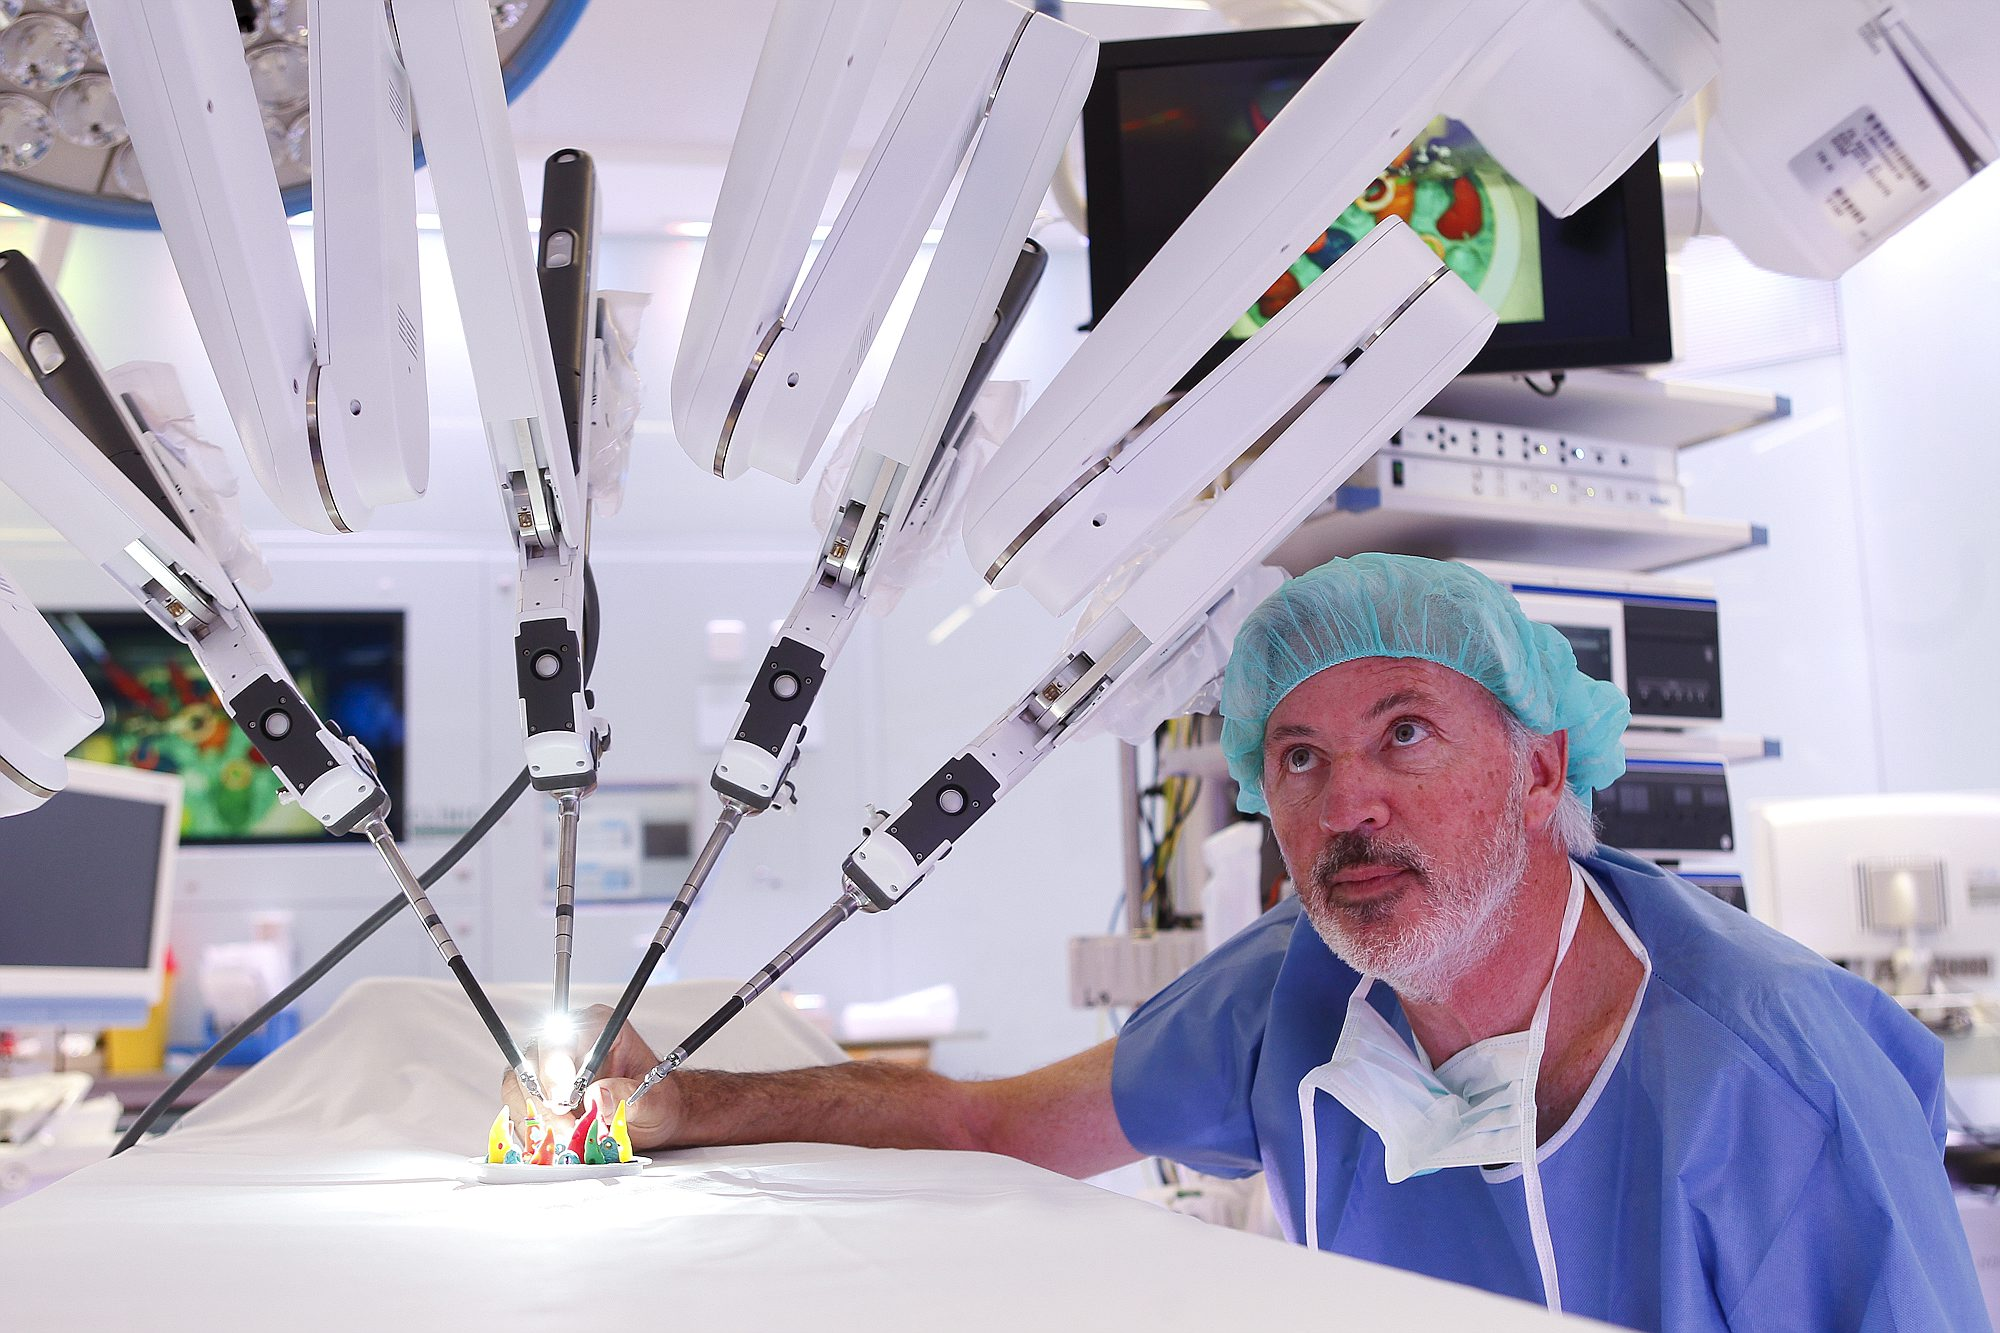
\includegraphics[width=0.8\textwidth]{Antonio_M_Lacy.jpg}
                     \caption{Les organes terminaux de DaVinci : des outils précis}
                     \label{fig:davinci}
                 \end{figure}                
                 
            \subsubsection{Wandercraft}
                
                \paragraph{}
                    Un nombre important de personnes handicapées, hémiplégiques, tétraplégiques ou 
                    ayant des déficiences nerveuses sont dans l'incapacité totale de marcher, 
                    ou même de se tenir droit. En plus d'être privés de cette activité qui 
                    permet d'entretenir une grande partie des muscles dorsaux et abdominaux, 
                    ces personnes peuvent également ressentir une exclusion sociale du fait 
                    de l'incapacité de se tenir debout. 
                    
                \paragraph{}
                    Pour pallier à ces problèmes, un certains nombre d'entreprises proposent
                    des solutions technologiques : orthèses, verticalisateurs ou même exosquelettes. 
                    Nous nous intéresserons ici à la start-up française Wandercraft (qui a 
                    acueilli l'auteur pour son stage de 4\^{ème} année). 
                    Wandercraft développe un exosquelette de marche, qui se présente sous la forme 
                    d'un squelette robotisé qui vient se fixer à l'extérieur des jambes du patient, 
                    comme on peut le voir sur la figure \ref{fig:wdc}.
                
                \begin{figure}[h!]
                    \centering
                    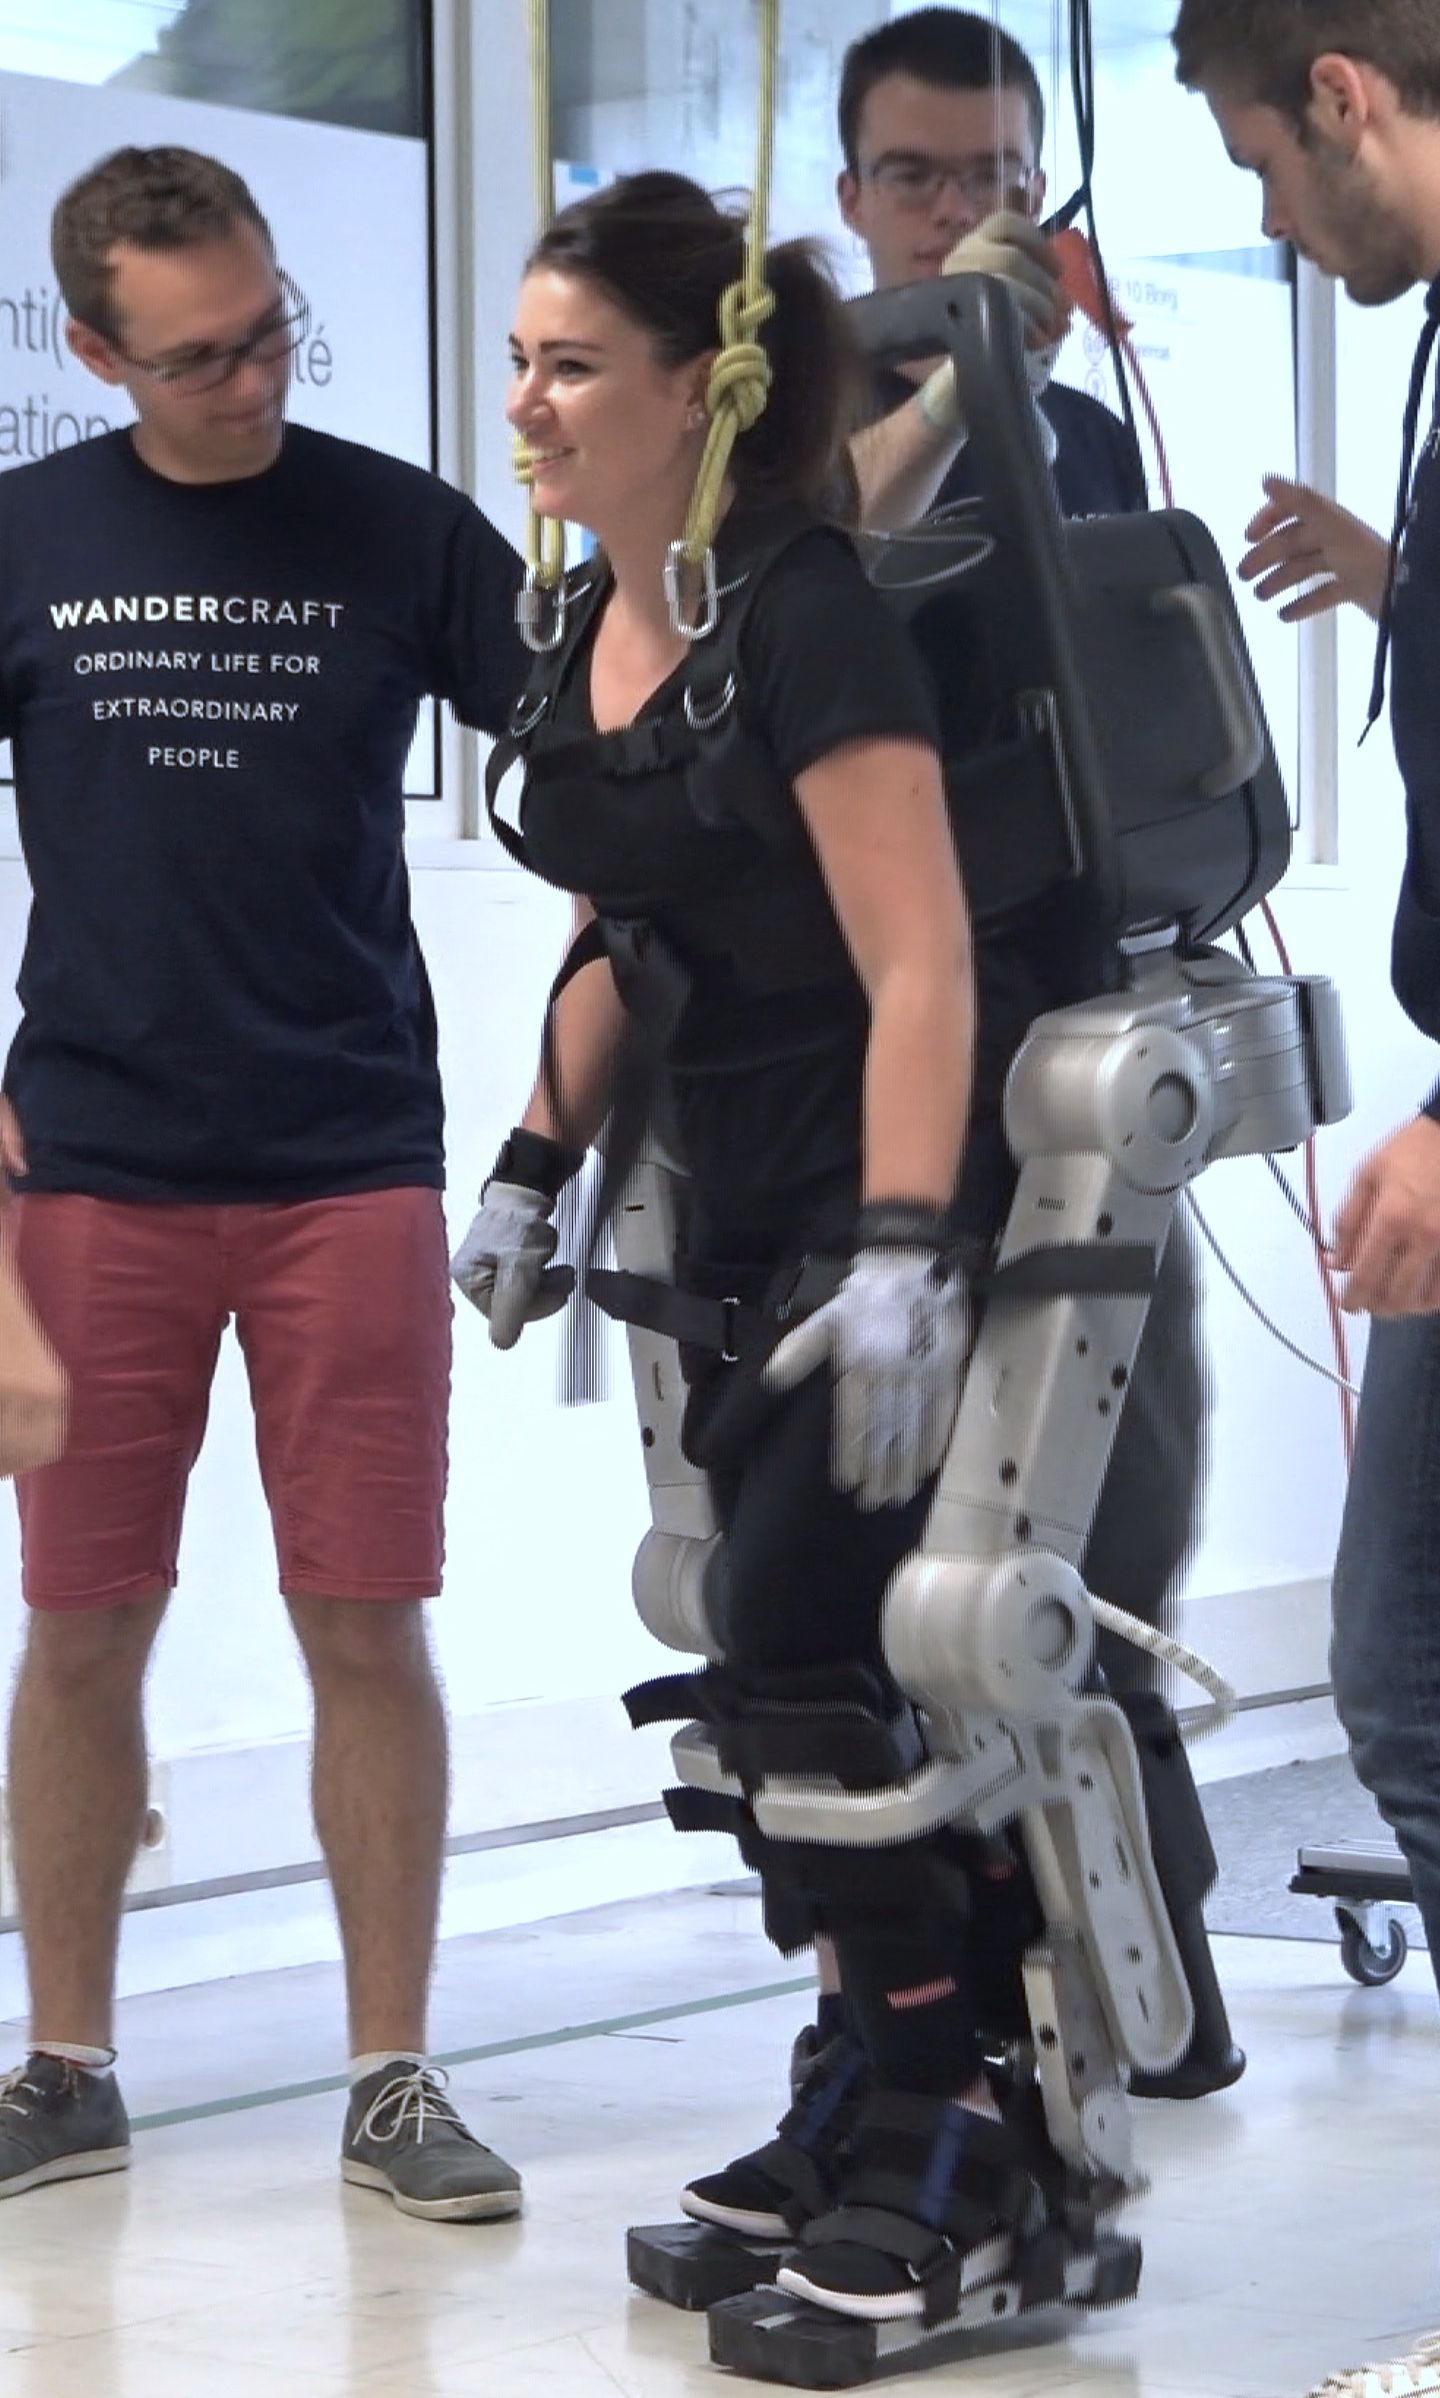
\includegraphics[width=0.5\textwidth]{wandercraft-exosquelette.jpg}
                    \caption{Atalante de Wandercraft, l'exosquelette faisant remarcher les personnes handicapées}
                    \label{fig:wdc}
                \end{figure}
                
                \paragraph{}
                    Wandercraft propose une rupture technologique complète avec les orthèses 
                    et verticalisateurs, en créant un exosquelette qui sera, à terme, utilisable 
                    quotidiennement et dans n'importe quel environnement. La spécificité technique qui 
                    caractérise Atalante - l'exosquelette - est son modèle de marche : 
                    la marche se veut proche de la marche humaine, à la fois dans la position 
                    du corps patient et dans le mouvement même. 
                    
                \paragraph{}
                    Atalante est en fait le premier exosquelette de marche dynamique au 
                    monde. Voué à être dans un premier temps distribué à des centres de 
                    soins, un accent particulier est mis sur le développement d'un système 
                    permettant à la personne handicapée de réaliser exactement les mêmes mouvements 
                    de marche qu'une personne non-handicapée. 
                    
                \paragraph{}
                    On approche ici un domaine de la robotique de service assez original, 
                    car l'humain devient partie constituante du robot, et est intégré 
                    au modèle de ce dernier. Si la marche est une phénomène complexe 
                    à modéliser et à maîtriser, on peut tout de même observer le même 
                    type d'innovation pour des prothèses de bras ou de main robotisées.
                    
        
    \section{Les robots mobiles, acteurs de leurs environnements}
        \subsection{Terrestre}
            \paragraph{}
                Un robot mobile terrestre évolue sur un plan. 
                Pour être omnidirectionnel, un robot mobile terrestre 
                doit posséder 3 degrés de liberté : 
                \begin{itemize}
                    \item une translation selon les deux axes formant la base
                    du plan, 
                    \item une rotation selon la normale du plan. 
                \end{itemize}
                
            \paragraph{}
                On se rend compte que la morphologie d'une voiture 
                (deux roues dirigées, plusieurs roues motrices) ne lui permet 
                d'avoir que 2 degrés de liberté : une rotation selon 
                la normale de la route et une translation. Ainsi, elle n'est 
                pas omnidirectionnelle, c'est donc pour cela qu'il est nécessaire 
                de réaliser des manoeuvres pour se placer dans une position 
                et orientation précise. 
                
            \paragraph{}
                Il en est de même pour la base roulante du robot utilisé
                par le club robot de l'INSA Toulouse : le déplacement se 
                fait grâce à deux roues motrices, utilisées en différentiel
                pour tourner. 
                
            \paragraph{}
                Il est cependant possible de créer des plateformes omnidirectionnelles, 
                en utilisant des roues caddy ou suédoises. 
                
            \paragraph{}
                Les roues caddy sont en fait les roues pivotantes que l'on 
                trouve par exemple sur les caddy de supermarché.
                Lorsque l'on applique une force quelconque, dirigée 
                parallèlement au plan sur lequel le caddy se déplace, les roues
                pivotent et s'orientent de manière à minimiser la force de 
                résistance du caddy. Elles se mettent donc dans la direction 
                de la force appliquée. Ainsi, le caddy peut être déplacé dans 
                n'importe quelle position $(x, y, \theta)$ sans manoeuvre. 
                
            \paragraph{}
                Les roues suédoises permettent également cette liberté. Ce sont en
                fait des roues dont les pneus sont eux-mêmes des roues. 
                Lorsqu'une telle roue est actionnée, elle génère deux forces 
                : une dans la direction "classique" de la roue, et une selon l'axe 
                de rotation de la roue (la direction de cette force dépend de la
                morphologie de la roue). 
                
            \paragraph{}
                Prenons l'exemple d'un véhicule possédant 4 roues (par exemple, une 
                voiture). En commandant ces roues de manière couplée, la résultante des 
                forces peut entraîner une translation selon 
                l'axe "avant/arrière" ou l'axe "droite/gauche" du véhicule. 
                En commandant les roues de manière différentielle, on peut faire tourner
                le véhicule sur place. 
                On a un véhicule possédant 3 degrés de liberté, qui est donc omnidirectionnel.
                
            \paragraph{}
                Un autre type de robot mobile terrestre existe : les robots à pattes. Ceux-ci seront 
                abordés dans la section suivante.
                
        \subsection{Robotique terrestre à pattes, robotique bipède}
            \paragraph{}
                Certains robots ont une architecture inspirée directement du règne animal : 
                des robots à pattes comme Big Dog, des robots bipèdes comme Atlas ou HRP-2. 
                La commande de ces robots est complexe, car elle doit reproduire les comportements 
                effectués par le cortex moteur animal pour garder l'équilibre. Dans la suite 
                de cette section, nous nous intéresserons essentiellement à la robotique bipède. 
            
            \paragraph{}
                Dans le cas de la robotique bipède, le contrôle est complexe. En 1968, Miomir Vukobratović
                présente lors du \textit{Troisième Congrès de l'Union pour la Mécanique Théorique et Appliquée} un 
                concept mathématique : le \textit{Z.M.P.} ou \textit{Zero Moment Point}. Pour un robot
                humanoïde, il s'agit grossièrement des points pour lesquels le moment est nul. 
                
            \paragraph{}
                Ce moment est dû au poids du robot, aux frottements entre le pied et le sol et à d'éventuelles
                interaction avec l'environnement extérieur. Lorsque le robot est sur un seul pied, ce point
                est unique. 
                
            \begin{figure}[h!]
                \centering
                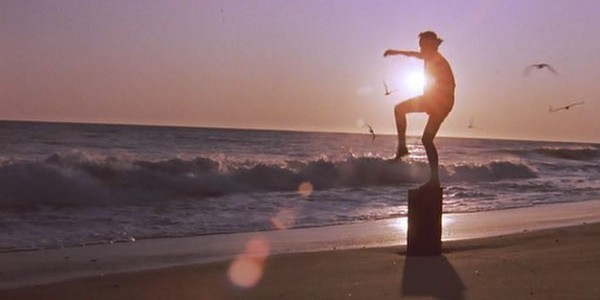
\includegraphics[width=0.8\textwidth]{karate_kid_1984.jpg}
                \caption{Une question d'équilibre et de placement du Z.M.P. (\textit{Karate Kid}, 1984)}
                \label{fig:danielsan}
            \end{figure}
                
                
            \paragraph{}
                Étudions maintenant l'intérêt du positionnement de ce point. Pour cela, nous allons utiliser
                un exemple tiré sur film "Karaté Kid", lorsque Daniel-san s'entraîne à tenir en équilibre sur 
                un seul pied (voir figure \ref{fig:danielsan}). 
                

            \paragraph{}
                On peut imaginer que toutes les forces qui s'appliquent sur lui 
                créent un moment au niveau de son pied. Lorsqu'il se tient droit et maîtrise son 
                équilibre, les composantes du moment selon les axes définissant la base du sol 
                sont nulles : Daniel-san est en équilibre, et ne bascule pas en avant ou sur le côté. 
                
            \paragraph{}
                Il existe une explication à cet équilibre : si le \textit{Z.M.P.} correspond à 
                l'endroit d'application d'une force qui ferait "tourner" le jeune karatéka au niveau 
                de son pied par rapport au sol, alors le fait de placer ce \textit{Z.M.P.} dans 
                l'enveloppe convexe du pied lui permettra de tenir en équilibre. 
                
            \paragraph{}
                C'est exactement ce principe qui est utilisé pour certains modèles de marche bipède,
                qui utilisent la planification du \textit{Z.M.P.} pour prévoir où placer les pieds 
                de manière à être toujours stables. Il est possible qu'il s'agisse de ce que l'on peut observer 
                sur les vidéos mettant en scène le robot Asimo de Honda en train de marcher. 
        
            \paragraph{}
                La limitation de la marche en planification du \textit{Z.M.P.} réside en la quasi-perpétuelle
                staticité du robot. Une autre école de marche souhaite se rapprocher de la marche dynamique 
                que l'on peut observer chez l'humain, en utilisant une méthode appelée \textit{Hybrid Zero Dynamics}. 
                
            \paragraph{}
                Cette méthode s'applique aux robots bipèdes sous-actionnés, c'est-à-dire les 
                robots qui possèdent au moins un degré de liberté non-actionné (généralement 
                l'interface pied-sol). 
                
            \paragraph{}
                Vulgairement, le principe de cette méthode de marche est de déséquilibrer le robot vers l'avant, 
                puis de venir placer les pieds de manière à rattraper l'équilibre du robot, tout en le laissant
                préserver une dynamique "vers l'avant". Si l'on considère notre robot bipède comme un système 
                non-linéaire, la première étape est d'emmener le robot en dehors de son domaine de stabilité 
                (donc sortir le \textit{Z.M.P.} de l'enveloppe convexe du pied), puis d'actionner les jambes 
                de manière à faire converger le robot vers un cycle limite dont la vitesse moyenne est constante. 
                
        \subsection{Robotique sous-marine et aérienne} 
            \paragraph{} 
                Cette section croise à la fois la robotique sous-marine et aérienne, 
                car ces deux domaines de la robotique mobile sont proches en terme
                de degrés de liberté et donc de solutions. 
                
            \paragraph{}
                Les robots sont ici en immersion dans un fluide, et doivent donc 
                posséder les 6 degrés de liberté d'un solide dans l'espace 3D pour
                être omnidirectionnels. 
                
            \paragraph{}
                Parmi les robots aériens fameux, certains ont obtenu un fort intérêt 
                de l'industrie et du secteur militaire : les drones. Ces robots, 
                autonomes ou télé-opérés, voient leur nombre d'applications 
                augmenter. 
                
            \paragraph{}
                Il serviront peut être demain à livrer nos colis, transporter 
                notre courrier, surveiller nos forêts, ... 
                
                        
    \section{Morphologie, architecture et commande des robots manipulateurs}
        \subsection{Les robots manipulateurs sériels}
            \subsubsection{Présentation}
                \paragraph{}
                    Parmis les robots manipulateurs, certains (souvent
                    appelés "bras manipulateurs") sont composés de moteurs 
                    agencés \textit{les uns après les autres}. Le manipulateur
                    présenté en figure \ref{fig:robotarm} est constitué de moteurs en série actionnant
                    les articulations A, B et C (de la base vers l'extrémité), composant une chaîne cinématique ouverte. 
                    
                    
                \begin{figure}[h!]
                    \centering
                    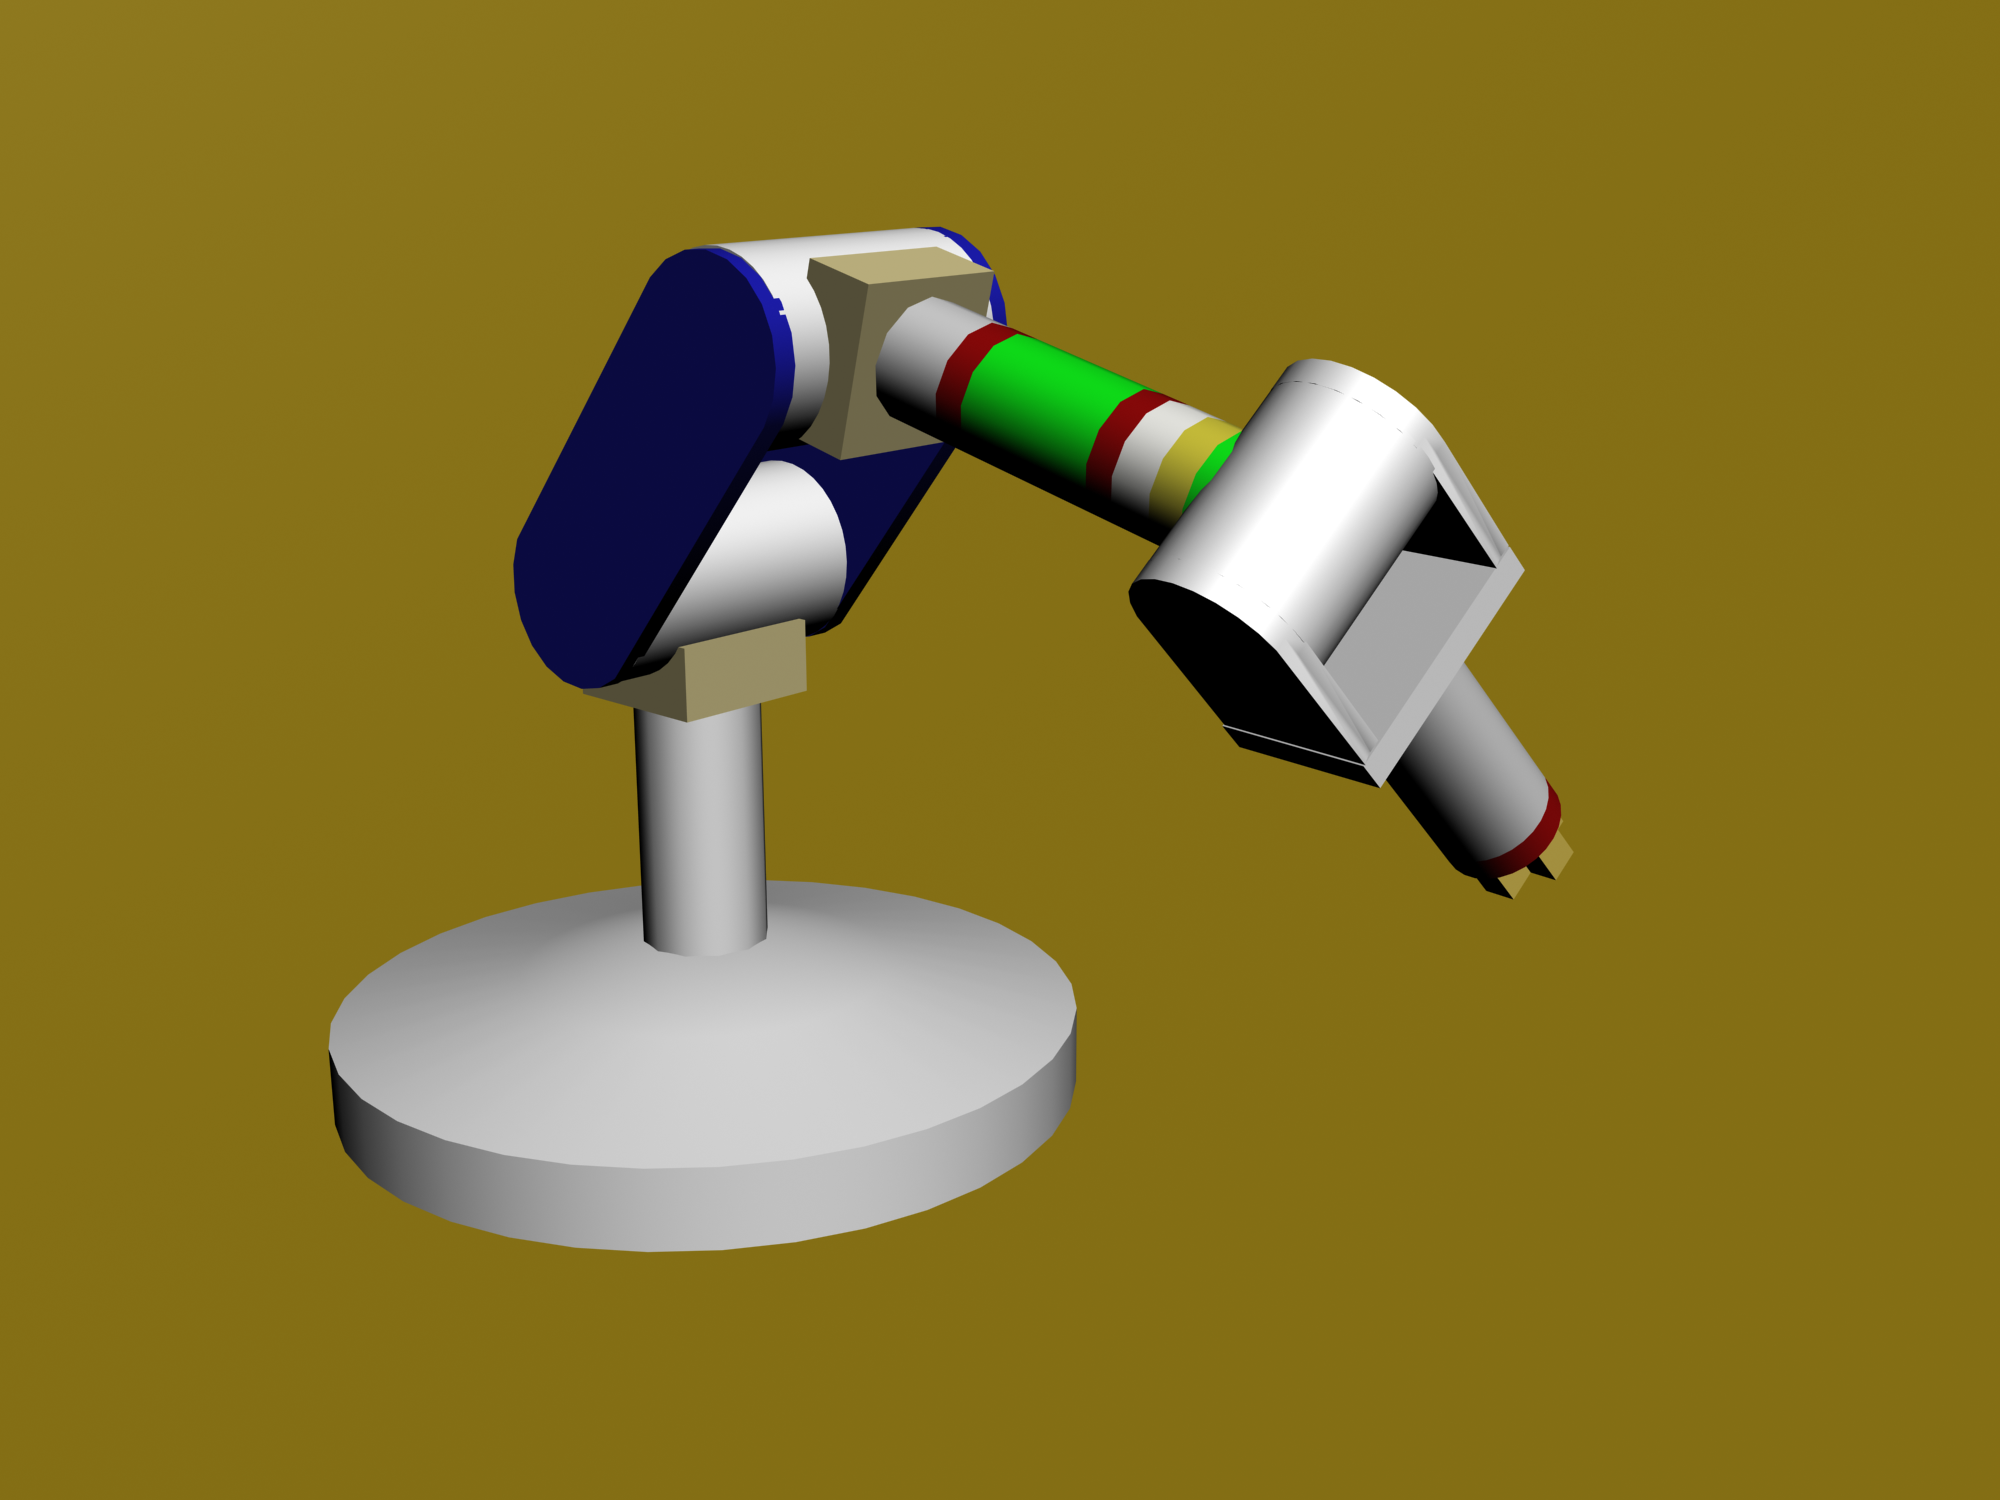
\includegraphics[width=0.5\textwidth]{Robot_arm_model_1.png}
                    \caption{Représentation cinématique d'un robot manipulateur à 5 degrés de liberté} 
                    \label{fig:robotarm}
                \end{figure}
                    
                \paragraph{}
                    On s'aperçoit sur cette figure que la position de 
                    l'articulation A influe sur la position des articulations
                    B et C. La commande des trois articulations est donc couplée, 
                    c'est-à-dire qu'il faut par exemple prendre en compte les positions
                    de A et B pour asservir la position de M (l'extémité) en déplaçant uniquement
                    C. 
            
                \paragraph{}
                    Si cette solution paraît simple, le couplage des articulations est
                    néanmoins source de nombreux problèmes.
                    
            \subsubsection{Architecture} 
                \paragraph{}
                    En terme de degrés de liberté, plusieurs choix sont possibles 
                    pour les robots sériels. 
                    Une architecture très commune en industrie est l'architecture
                    SCARA. Certains robots manipulateurs possèdent plus de degrés de
                    liberté que nécessaire, leur permettant ainsi de changer de configuration. 
                    
                \paragraph{}
                    SCARA signifie Selective Compliance Articulated Robot Arm. Il s'agit 
                    d'une architecture de chaîne cinématique spécifique, composée
                    de deux liaisons pivot chaînées, et reliées à la base par une 
                    liaison glissière (voir figure \ref{fig:scara}). 
                    
                    
                \begin{figure}[h!]
                    \centering
                    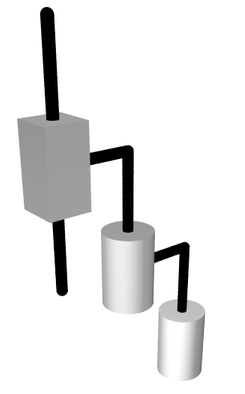
\includegraphics[width=0.2\textwidth]{600px-SCARA_configuration.png}
                    \caption{La configuration cinématique de l'achitecture SCARA}
                    \label{fig:scara}
                \end{figure}
                
                \paragraph{}
                    Cette architecture permet par exemple au robot de travailler précisément
                    dans un plan dont la hauteur est définie au niveau de la liason glissière. 
                    Ces robots sont généralement assez précis car les deux liaisons pivot 
                    sont axées parallèlement au plan de travail, ce qui permet aux articulations
                    de ne pas avoir à supporter dans l'actionnement la masse du reste du bras. 
                    
                \paragraph{}
                    Certains robots sériels possèdent également plus de degrés de liberté 
                    que nécessaire (on parle alors de redondance). Par exemple, le bras manipulateur
                    PA10 construit par Mitsubishi (et dont l'architecture logicielle et matérielle
                    est \textit{open source}) possède 7 degrés de liberté, donc plus que les 
                    6 nécessaires dans l'espace en 3 dimensions. 
                    
                \paragraph{}
                    En contraignant dans la commande du robot certains degrés de liberté, on créé
                    une configuration spécifique, dont il est évidemment possible de changer. Cette 
                    redondance permet donc d'obtenir un robot fortement générique, d'où son intérêt  
                    pour la communauté scientifique. 
                
            \subsubsection{Limitations}     
                \paragraph{}
                    Tout d'abord, les articulations
                    les plus proches de la base doivent être capable de supporter la masse 
                    des segments plus éloignés : 
                    
                    \begin{itemize}
                        \item A doit supporter les masses des segments $\left[AB\right]$, $\left[BC\right]$ et 
                        $\left[CM\right]$ 
                        \item B doit supporter les masses des segments $\left[BC\right]$ et $\left[CM\right]$. 
                    \end{itemize}
                    
                    Ceci influe fortement le dimensionnement du manipulateur si les moteurs
                    ne sont pas déportés. 
                
                \paragraph{}
                    La déportation des moteurs, qui paraît être la solution au problème précédent, 
                    permet d'introduire une autre caractéristique négative des robots sériels. 
                    Comme les positions des articulations sont couplées, la perte de précision ou de 
                    vitesse sur l'une d'entre elles influe sur les performances générales du système. 
                    
                \paragraph{}
                    Par exemple, la déportation des moteurs exige l'utilisation de courroies flexibles 
                    (ou d'un autre élément de transport d'énergie mécanique), dont les performances 
                    sont limitées. Ainsi, si le moteur est déporté, l'articulation perd en performances, 
                     donc toute la chaîne cinématique perd en performances. 
                     
                     
                \paragraph{}
                    Au delà des limitations physiques de ce type d'agencement, on trouve également des 
                    problèmes pour la commande des robots sériels. En effet, ces derniers peuvent conduire à des 
                    singularités mathématiques pour lesquelles plusieurs mouvements des articulations 
                    sont possibles pour réaliser un même déplacement de l'organe terminal. 
                    
                \paragraph{}
                    Prenons l'exemple du bras humain, qui peut être vu comme un robot manipulateur 
                    sériel. Lorsque nous souhaitons déplacer un objet d'un point A à un point B, 
                    nous pouvons le faire de plusieurs manières différentes : en avançant \textit{plus ou 
                    moins} l'épaule, en levant \textit{plus ou moins} le coude, en tournant \textit{plus 
                    ou moins} le poignet. 
                    
                \paragraph{}
                    On se rend donc bien compte qu'il existe une infinité de mouvements possibles 
                    pour déplacer notre objet du point A au point B. 
                    Cependant, comment choisir une trajectoire ? 
                    Cette tâche, réalisée naturellement par le cerveau 
                    chez l'humain, doit donc être explicitement décrite dans le cas d'un robot sériel. 
                    Il est également possible d'éviter de se placer dans des positions conduisant à 
                    des singularités. 
                
        \subsection{Les robots parallèles}
            \paragraph{}
                Pour pallier à certains problèmes des robots sériels, comme le manque de 
                précision ou de force du au chaînage des articulation, une autre typologie
                a vu le jour. 
                
            \paragraph{}
                Il s'agit des robots parallèles, possédant une chaîne cinématique fermée, 
                et dont chaque chaîne cinématique reliant la base à l'organe terminal 
                est indépendante. Les degrés de liberté, plutôt que d'être chaînés, sont
                donc accumulés en parallèle. 
                
            \paragraph{}
                En se rappelant que, dans un manipulateur sériel, chaque articulation
                doit supporter la masse de tous les segments la reliant à l'organe terminal, 
                on se rend bien compte qu'un robot sera plus fort, rapide et précis si
                ses chaînes cinématiques indépendantes sont plus courtes et plus nombreuses. 
                
            \paragraph{}
                Une application qui a nécessité la mise en place de ce genre d'architecture 
                est l'Usinage Grande Vitesse (ou \textit{U.G.V.}).
                
            \paragraph{}
                Lors d'une opération de fraisage d'un acier, la vitesse de déplacement
                de la fraise dans l'acier est limitée car, au-delà d'un certain seuil, 
                l'acier n'est plus découpé mais arraché. Cependant, il existe un second 
                seuil de vitesse de déplacement au-delà duquel l'usinage redevient possible. 
                
            \paragraph{}
                Les robots sériels ne possède pas la capacité de dépasser ce seuil, ce qui 
                à motivé la recherche d'une nouvelle typologie dans les années 1980. 
                
            \paragraph{}
                C'est cette architecture parallèle qui a été mise en place sur les robots 
                DELTA à 3 degrés de liberté, utilisés dans l'industrie suisse pour mettre 
                3 chocolats en boîte par seconde. L'architecture est tellement performante 
                que la vitesse de travail est uniquement limitée par le temps de préhension. 
                
            \begin{figure}
                \centering
                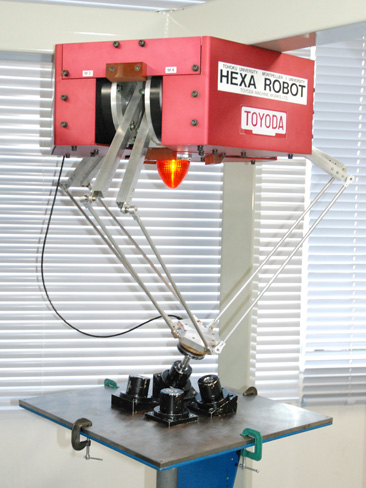
\includegraphics[width=0.5\textwidth]{M-1994-3_011.jpg}
                \caption{Le robot HEXA, et son architecture parallèle à 6 d.d.l.}
                \label{fig:hexa}
            \end{figure}
                
            \paragraph{}
                Cette typologie est reprise par le robot HEXA (figure \ref{fig:hexa}, conçu par l'université 
                de Tohoku à Sendai (Japon) et le groupe Toyoda, possédé par le géant Toyota. 
                Cependant sur HEXA, les chaînes d'actionnement sont doublées, et les chaînes 
                cinématiques ajoutées sont un peu écartées de celle initialement présente. 
                
            \paragraph{}
                On a donc, en plus des 3 degrés de liberté initiaux, 3 degrés de liberté
                supplémentaires qui permettent un contrôle total de l'organe terminal, 
                à savoir les 3 translations et 3 rotations. 
                
            \paragraph{}
                Il est intéressant de savoir que l'architecture parallèle, basée sur 
                l'utilisation de vérins, permet d'actionner des simulateurs mobiles 
                en tout genre. 
    
    \section{De l'intelligence des robots}
        \subsection{Positionnement du problème}
            \paragraph{}
                On a pu voir précédemment que dans certaines situations appelées 
                singularités, le robot manipulateur sériel doit choisir une trajectoire parmi une 
                infinité de mouvements possibles. 
                Si nous considérons notre propre bras comme un manipulateur sériel, et que 
                nous admettons qu'il présente les mêmes problèmes de singularité, comment l'être 
                humain choisit-il une trajectoire particulière ? 
                
            \paragraph{}
                Le fait d'avoir un cerveau, et donc d'être doués d'intelligence, nous permet 
                d'éviter simplement et intuitivement des problèmes très complexes à résoudre
                mathématiquement. 
            
            \paragraph{}
                Notre intelligence conditionne également notre interaction avec l'environnement, 
                et notamment avec les autres humains. Si l'Homme souhaite utiliser des 
                robots de service au quotidien, interagir ou même vivre avec eux, il va
                donc être amené à créer une forme d'intelligence pour ces robots. 
            
            \paragraph{}
                
                
        \subsection{Les méthodes d'apprentissage}
            \subsubsection{Machine Learning}
                \paragraph{}    
                    Le \textit{machine learning} (en français \textit{apprentissage automatisé}) est un 
                    domaine de l'intelligence artificielle visant à optimiser un modèle général pour une tâche 
                    particulière. Cette optimisation est appelée \textit{apprentissage}. 
                    
                \paragraph{}
                    Cette méthode diffère des autres méthodes utilisées en intelligence artificielle, car 
                    on ne cherche pas à modéliser parfaitement \textit{à priori} ce que doit faire le système, 
                    mais plutôt à le faire apprendre à partir d'exemples ou de réponses de son environnement. 
                    Ainsi, le \textit{machine learning} s'inspire des grands principes de l'évolution naturelle
                    (les systèmes s'adaptent à leur environnement) et l'applique au domaine de l'intelligence 
                    artificielle. 
                    
                \paragraph{}
                    Parmis les modèles couramment utilisés en \textit{machine learning}, on peut citer les 
                    KNN (\textit{K-nearest neighbors}), les SVM (\textit{Support Vector Machine}), et bien 
                    sûr les réseaux de neurones fortement utilisés aujourd'hui. 
                    
                \paragraph{}
                    On peut également utiliser des modèles d'ontologie pour stocker et représenter une
                    hiérachisation des données apprises. Ceci est basé sur une description hiérachique logique
                    des interactions entre différents concepts. 
                    
            \subsubsection{Réseaux de neurones et deep learning}
                
                \paragraph{}
                    Les réseaux de neurones sont une modélisation mathématique simple, utilisant
                    des entités élémentaires (\textit{neurones}) possédant une sortie et plusieurs entrées. 
                    Le neurone somme ses entrées et applique une fonction d'activation pour 
                    générer sa sortie. Un réseau de neurone utilise de milliers, millions voir milliards de ces entités, 
                    connectées les unes aux autres par couche de neurones. 
                    
                \paragraph{}
                    Si le lecteur peut retrouver dans la terminologie propre à ce 
                    domaine des mots tirés de la biologie, il ne faut cependant pas penser que 
                    le but des réseaux de neurones généralement utilisés est de fournir une modélisation fidèle 
                    du fonctionnement du cerveau. Il s'agit plutôt d'une modélisation grossière, 
                    permettant d'approximer n'importe quelle fonction non-linéaire (ce sont des 
                    \textit{approximateurs universels}). 
                    
                \paragraph{}
                    Certains réseaux de neurones sont tout de même utilisés pour 
                    leur plausibilité : c'est notamment le cas des \textit{spiking neural networks}, 
                    utilisant une modélisation fidèle du fonctionnement électrique 
                    des neurones pour résoudre des tâches. 
                    
                \paragraph{}
                    Il ne s'agit cependant pas là des modèles les plus utilisés. 
                    Les réseaux de neurones utilisés couramment sont assez semblable
                    à celui présenté sur la figure \ref{fig:mlp}. Ils se composent 
                    d'une couche d'entrée, une ou plusieurs couches cachées et une couche de 
                    sortie. 
                    
                \paragraph{}
                    Les poids reliant la sortie d'une couche aux entrées de la couche 
                    suivante sont des paramètres qui sont optimisés lors d'une phase 
                    appelée "apprentissage" (ou \textit{training}). 
                    Durant cette phase, on utilise généralement un jeu d'entrées/sorties. 
                    En comparant la sortie attendue avec la sortie de notre modèle, on
                    est capable de modifier les poids reliant les couches de manière à 
                    faire converger, tout au long de l'apprentissage, la sortie du modèle vers 
                    la sortie attendue. 
                
                \paragraph{}
                    La réelle force des réseaux de neurones réside dans leur capacité 
                    à généraliser. Si l'apprentissage est stoppé assez tôt (\textit{early stop}, permettant
                    d'éviter l'\textit{overfitting}, le sur-apprentissage), le modèle 
                    est capable : 
                    \begin{itemize}
                        \item de répondre presque correctement lorsque l'on lui passe une entrée du jeu 
                        de données, 
                        \item de répondre presque correctement lorsque l'on lui passe une entrée qui ne 
                        fait pas partie du jeu de données. 
                    \end{itemize}
                    Cela veut dire que ces réseaux peuvent, à partir d'une faible quantité de données 
                    caractérisant un phénomène, d'extraire les concepts principaux de manière à généraliser 
                    et modéliser ce phénomène. 
                    
            
                \begin{figure}[h!]
                    \centering
                    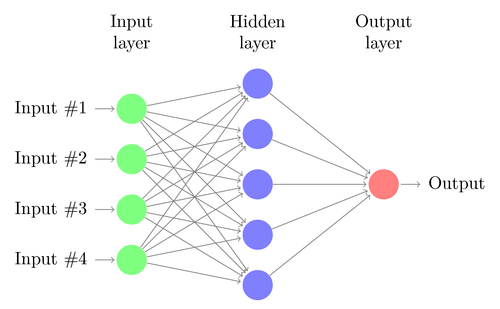
\includegraphics[width=0.5\textwidth]{neural-network.png}
                    \caption{Un réseau de neurones à trois couches successives, appelé "perceptron multi-couches"}
                    \label{fig:mlp}
                \end{figure}
                    
                    
                \paragraph{}
                    Un des hyperparamètres important des réseaux de neurones est la capacité du réseau, qui 
                    dépend du nombre de neurones présent. La capacité influe sur la faculté d'un réseau
                    à approximer une fonction précisément. On peut intuitivement se dire que plus la capacité 
                    sera grande, plus le réseau pourra approximer une fonction précisément. Ceci est totalement 
                    faux : la capacité d'un réseau de neurones doit correspondre avec la complexité de la fonction, 
                    comme on peut le constater en figure \ref{fig:overfit}. 
                    
                \begin{figure}[h!]
                    \centering
                    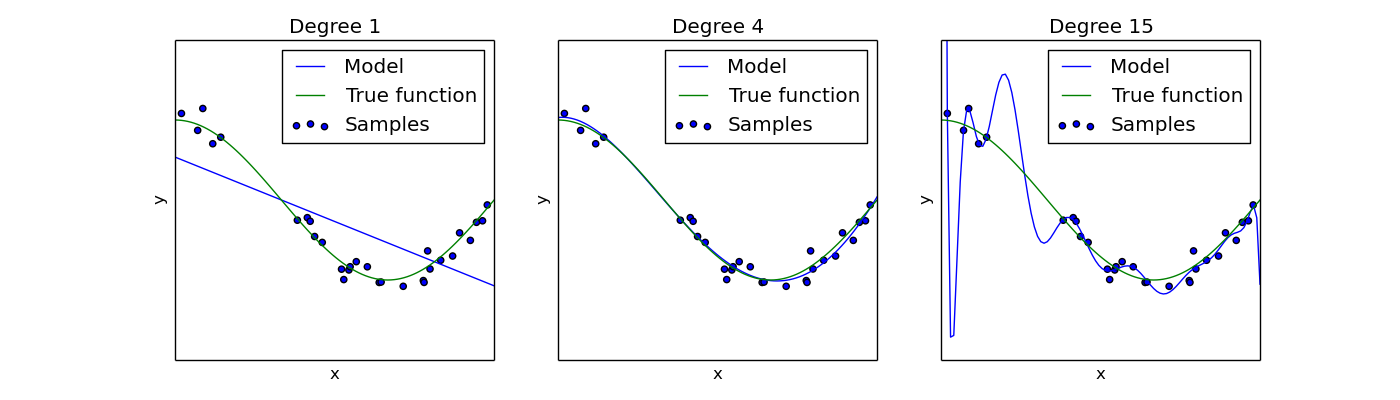
\includegraphics[width=\textwidth]{plot_underfitting_overfitting_0011.png}
                    \caption{De gauche à droite : une capacité trop faible, correcte et trop élevée pour la tâche.}
                    \label{fig:overfit}
                \end{figure}
                
                
                \paragraph{}
                    Cette idée d'utiliser des d'unités génériques performant une simple opération dans 
                    des réseaux pour générer ou appréhender des comportements complexes date de 1943 
                    (McCulloch et Pitts). Ceci a connu un fort essor jusqu'aux années 1980 (avec la 
                    création du néocognitron de Kunihiko Fukushima, réseau de neurones proche des 
                    architectures modernes). 
                    
                \paragraph{}
                    On se rend alors vite compte du problème de sur-apprentissage, et de la 
                    difficulté de réaliser des réseaux de neurones de très grande capacité. 
                    Arrive alors une stagnation dans le domaine, malgré quelques avancées 
                    comme la création réseaux de neurones convolutionnels par Yann Le Cun
                    (aujourd'hui directeur du groupe de recherche en IA de Facebook). 
                    C'est en 2012 que, sur les travaux de Le Cun,  A. Krizhevsky, I. Sutskever, et G. E. Hinton
                    publient "Imagenet classication with deep convolutional neural networks". 

                \paragraph{}
                    Dans cette publication, les auteurs réussissent à créer et entraîner un réseau 
                    de neurones dit \textit{profond} (d'une grande capacité, d'où le \textit{deep learning}) 
                    pour classifier des images d'un énorme jeu de données avec une précision 
                    jamais égalée. 
                    
                \paragraph{}
                    Depuis lors, nous connaissons un essor considérable de l'intelligence 
                    artificielle, notamment chez les géants de l'Internet. C'est grâce à cela 
                    que Facebook est capable de proposer des identifications automatiques sur
                    des photos, ou que Google Assistant est capable de nous comprendre et 
                    d'interpréter nos questions.
                    
                \paragraph{}
                    Ces nouvelles innovations sont fortement prometteuses pour la robotique, 
                    dans le domaine de la vision ou de la plannification de trajectoire, 
                    mais aussi pour compenser les erreurs de modèles, lorsque que l'on transfert 
                    un programme fonctionnant en simulation sur un robot réel. 
            
            \subsubsection{Reinforcment learning et robotique développementale}
            
                \paragraph{}
                    Nous avons pu voir que le \textit{deep learning} offre des possibilités 
                    très larges (et encore inexplorées), mais un sous domaine de l'intelligence 
                    artificielle en particulier peut nous amener à remettre totalement 
                    en question la façon dont nous faisons de la robotique aujourd'hui. 
                    
                \paragraph{}
                    Ce domaine est l'apprentissage par renforcement (\textit{reinforcment learning}), 
                    et même plus spécifiquement l'apprentissage profond par renforcement (\textit{deep 
                    reinforcment learning}). 
                    
                \paragraph{}
                    Le principe est le suivant : 
                        \begin{itemize}
                            \item un agent (le programme apprenant) est en immersion dans 
                            un environnement dans lequel il peut agir, observer, et obtenir 
                            des récompenses,
                            \item l'agent essaie d'abord aléatoirement des actions, observe 
                            les réponses de l'environnement et les récompenses reçues,
                            \item l'agent est constitué d'un modèle interne, proche de ceux 
                            abordés précédemment, qui sert à prédire l'action et qui est constamment modifié pour maximiser 
                            la récompense reçue, 
                            \item au fur et à mesure de l'apprentissage, on laisse moins de place
                            aux actions aléatoires (\textit{exploration}), et plus aux actions
                            déterminées par le modèle (\textit{prédiction}). 
                        \end{itemize}
                        
                \paragraph{}
                    On observe alors, si la politique d'apprentissage est bien sélectionnée
                    et le modèle interne cohérent avec la tâche à réaliser, que l'agent apprend 
                    à analyser son environnement et à déterminer dans quel cas utiliser une action
                    particulière de manière à maximiser sa récompense. 
                    
                \paragraph{}
                    Si cela paraît un peu abstrait, le lecteur pourra se référer au très sérieux papier 
                    publié par un laboratoire de DeepMind : "Playing Atari with Deep Reinforcement Learning". 
                    Est présenté dans cette publication un modèle capable d'apprendre à dépasser l'humain 
                    sur des jeux Atari. 
                    
                \paragraph{}
                    Nous sommes encore ici dans le domaine du jeu vidéo, et non pas dans le
                    domaine de la robotique. Cependant, l'apprentissage par renforcement forme 
                    une partie de l'avenir de la robotique, comme peut le montrer \href{https://www.youtube.com/watch?v=gn4nRCC9TwQ}{cette vidéo} 
                    de l'IA de DeepMind qui apprend en simulation à marcher, à courir, et à 
                    garder son équilibre, ce sans base de savoir initial. 
                    
                \paragraph{}
                    En utilisant des outils comme ROS (\textit{Robot Operating System}) et 
                    Gazebo (outil de simulation lié à ROS), on peut créer des simulations
                    de robots, très fidèles à la réalité. Rien ne nous empêche alors 
                    d'utiliser l'apprentissage par renforcement pour apprendre, par 
                    exemple, au robot HRP-2 de marcher mieux que ce que nous saurions 
                    faire en utilisant une modélisation mathématique classique. 
                    
                \paragraph{} 
                    De plus, si nous arrivons à créer un système de valeur permettant 
                    à un robot de déduire des récompenses en observant l'environnement
                    (fonction réalisée par le complexe amygdalien chez l'Homme), il sera possible
                     de concevoir des robots qui apprennent tout au long de leur cycle de vie.
                     
                \paragraph{}
                    Peut-être donc que demain, le robot ne sera plus une machine fabriquée
                    spécifiquement pour une tâche mais une créature capable d'évaluer son environnement, 
                    une page blanche fournie avec des fonctions basiques, et l'incroyable faculté d'apprendre.
                    
            
    \newpage
    \section*{Conclusion}
        \paragraph{}
            La robotique est un secteur relativement récent, qui 
            possède un fort potentiel et succite un intérêt énorme pour 
            les communautés industrielle et scientifique. 
    
        \paragraph{}
            Fondamentalement, la robotique est une réponse de l'Homme à un objectif qu'il 
            a toujours eu, à savoir construire une créature douée de vie artificielle. 
            
        \paragraph{}
            Si certains robots sont déjà utilisés pour réaliser 
            des tâches ne présentant pas d'intérêt pour l'Homme 
            (\textit{robotique manufacturière}), un nouveau souffle 
            prône l'utilisation de robots au service de la société humain 
            (\textit{robotique de service}). 
            
        \paragraph{}
            Parmi les applications de la robotique de service, 
            on peut notamment citer celles dans le domaines médical.
            Exosquelettes, robots-chirurgiens : la robotique nous permet 
            d'apporter de nouvelles solutions à des problèmes anciens. 
            
        \paragraph{}
            La capacité d'un robot à intéragir avec l'environnement
            peut, dans certains cas, être quantitativement décrite à 
            travers la notion de degrés de liberté. 
            
        \paragraph{}
            Nous avons vu dans une dernière partie qu'il est possible 
            que demain, le robot soit un être doté d'intelligence, 
            et d'un système de valeur comme le notre. 
            
        \paragraph{}
            Ceci impose des considérations éthiques et des réflexions qui 
            doivent être menées avant même de créer des solutions 
            techniques. Si nous créons un être proche de l'Homme, 
            que nous le dotons d'intelligence, quels seront ses droits légitimes ? 
    
\end{document}
